\section{$S= 3/2$ Thermometry}\label{spin1.5-thermo}
We consider again the V2 Silicon vacancy which due to the 4H-SiC trigonal
pyramidal symmetry has a stable ground state ZFS with respect to temperature and can not be used for thermometry \cite{Castelletto_2024}.
However, the ZFS of the excited state of the Silicon vacancy has a much
larger change rate with the temperature compared with the
dD/dT of the ground state of the divacancy in 4H-SiC or the
NV centre in diamond \cite{Anisimov2016}.

% This can be a promising tool for
% thermometry, although the change of the ZFS of the excited
% state can not be detected directly from the ODMR spectrum
% due to the short lifetime of the excited state. As discussed
% in the magnetometry section, in the vicinity of the LAC, the
% PL intensity reaches a local extreme point [28]. By adding a
\begin{wrapfigure}{l}{0.37\textwidth}%
	\centering%
	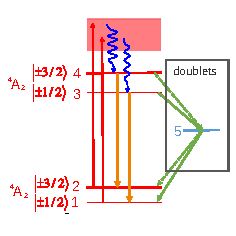
\includegraphics[width=0.37\textwidth]{figures/actual-stokes.pdf}
	\caption{Adapted from Wang et al.}\label{fig:stokes}
\end{wrapfigure}%

Schemas have been developed which exploit the increase in photoluminescence in the vicinity of level anti-crossings to measure the change in the excited state $D$ as in the work by Anisimov et al.  

We will focus instead on an alternative all optical method which exploits the dependence on temperature of the photoluminescence of the spin system.

\begin{wrapfigure}{r}{0.4\textwidth}%
	\centering%
	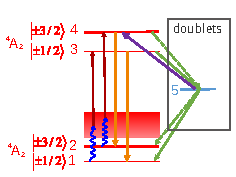
\includegraphics[width=0.4\textwidth]{figures/stokes.pdf}
	\caption{Adapted from Wang et al.}\label{fig:anti-stokes}
\end{wrapfigure}%

Anti-Stokes excitation is a process in which the wavelength of the exciting photon is longer (i.e. lower energy) than that
of the emitted photons (visualised in figure \ref{fig:anti-stokes}).  The mechanisms of anti-stokes excitation have been studied and include multiphoton absorption, phonon absorption, and Auger recombination
\cite{Tran2019, Wang2019}.

Since the anti-Stokes excitation process occurs with an energy contribution from the temperature dependent phonons,
the ratio between the anti-Stokes and Stokes photoluminescence intensity is proportional to the density of the phonons. 
The number density of the phonons obeys a Bose–Einstenin distribution \cite{Wang2018}
\begin{equation}
    \frac{I_{\ce{AS}}}{I_{\ce{S}}} \propto \exp\left\{\frac{\Delta E}{k_B T} -1 \right\}
    \label{eq:anti-stoke-ratio}
\end{equation}
where $I_{\ce{AS}}$ and $I_{\ce{S}}$ are the photoluminescence intensities for anti-Stokes and Stokes respectively for a datum laser power. $\Delta E$ represents the energy gap between the excitation photon and the zero phonon line i.e. the phonon contribution to the excitation. 

% When ∆E ≫ kB T,
% we approximately have IASPL /IPL ∝ exp(−∆E/kB T) [165].

We may reduce this to a temperature dependent exponential curve when $\Delta E \ll k_B T$ as \eqref{eq:anti-stoke-ratio} reduces to 
\begin{equation}
    \frac{I_{\ce{AS}}}{I_{\ce{S}}} \propto \exp\left\{\frac{\Delta E}{k_B T} \right\}.
    \label{eq:anti-stokes-ratio-reduced}
\end{equation}

Wang et al. analysed the anti-Stokes excitation of the Silicon vacancy \cite{Wang2021}. The zero phonon line for the defect is around $917$nm, so a Stokes excitation was induces by a laser with $1030 > 917$nm and the anti-Stokes excitation was induced by a laser with $720 < 917$nm. Using the same power for both lasers, the intensity of the photoluminescence from the anti-Stokes excitation increased as temperature increased. Conversely the intensity from the Stokes excitation decreased with temperature. The ratio therefore agrees with the statistical model in \eqref{eq:anti-stoke-ratio}. 

Thus to realise a thermometer, we fit data to \eqref{eq:anti-stokes-ratio-reduced} with measurable proportionality and correction factors $a, b, c, T_0$ as \cite{Tran2019}
\begin{equation}
    \frac{I_{\ce{AS}}}{I_{\ce{S}}} = a +  b\exp\left\{-\frac{c}{T - T_0} \right\}.
    \label{eq:}
\end{equation}

Temperature may then be inferred by solving the equation as 
\begin{equation}
    T = T_0 - \frac{c}{\ln\left(\left[{\frac{I_{\ce{AS}}}{I_{\ce{S}}} - a}\right]/b\right)}.
    \label{eq:anti-stokes-solution}
\end{equation}

For the SiC Silicon vacancy the intensity ratio, and thus the proposed thermometry sensitivity, is most sensitive at room temperature and above. 

\todo[color=red, inline]{Affects of other factors? e.g. $\vec{B}, \vec{E}$\cite{Wang2021}}


% \begin{figure}[H]
%     \begin{center}
%         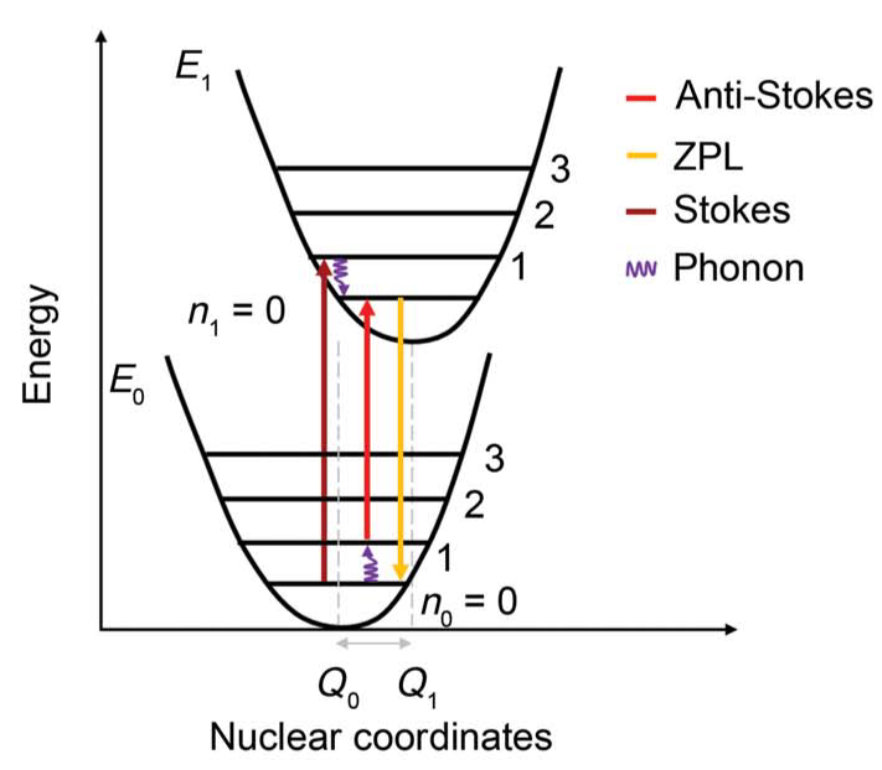
\includegraphics[width=0.4\textwidth]{figures/stokes.png}
%     \end{center}
%     \caption{}\label{fig:stokes}
% \end{figure}


\begin{summary}{$S=3/2$ Thermometry Summary}{sum:spin1.5thermo}
	We may achieve all optical thermometry using an $S = 3/2$ system provided:
	\begin{enumerate}
		\item We can identify three lines.
	\end{enumerate}
\end{summary}

